\documentclass[nosymbols]{beamer}	% Is better for some Windows user.
%
% For (excessive) usage in your document.
\newcommand{\docplace}{Magdeburg}
\newcommand{\docuniversity}{Otto-von-Guericke-Universit\"at Magdeburg} % Otto-von-Guericke-University Magdeburg.
\newcommand{\docuni}{OvGU}
\newcommand{\docfaculty}{Faculty of Computerscience} % Faculty of Computer Science.
\newcommand{\docfac}{INF}	% Important(!!!) for choosing the logo and colortheme. Available are:
% EIT GSE INF MATH MB MED NAT OVGU VST WW
\newcommand{\docinstitute}{Institute for Intelligent Cooperative Systems} % Department for Technical & Operational Information Systems.
\newcommand{\docinst}{IKS}
\newcommand{\docgroup}{Data and Knowledge Engineering Goup} % Data and Knowledge Engineering Goup.
\newcommand{\docgr}{ESS}
\newcommand{\docauthor}{Julian Scholle}
\newcommand{\docauthoremail}{jscholle@st.ovgu.de}
\newcommand{\doctitle}{Autonomous Driving in Urban Centers} % My awesome title.
\newcommand{\doctitleshort}{Kurztitel} % Short title.
\newcommand{\docsubtitle}{Roundabout Monitoring}
\newcommand{\docsubject}{Semantic Desktop}
\newcommand{\docplainkeywords}{Semantic Desktop, User Interface, Interface, Ontology, Exploration, Search} % For use in text.
\newcommand{\dockeywords}{ {Semantic Desktop} {User Interface} {Interface} {Ontology} {Exploration} {Search} } % Tagify metadata -> use package hyperref.
\newcommand{\docdate}{\today}				% Edit here author informations.
%\documentclass[nosymbols]{beamer} % Better in main.tex/Presentation.tex.
%
%\usepackage[ngerman]{babel}		% German headings.
\usepackage[T1]{fontenc}			% German typesetting.
\usepackage[utf8]{inputenc} 		%Universal/Linux Kodierung
%\usepackage[ansi]{inputenc} 		%Windows Kodierung
%\usepackage[applemac]{inputenc}	%MacOS Kodierung
%\usepackage[latin1]{inputenc} 		%Standart & Windows Kodierung
%
%\usepackage{lmodern}				% Better font encoding.
%\usepackage{verbatim} 				% Multiline Comments.

\usepackage{geometry}
\usepackage{graphicx}
\usepackage{subfigure}
%
\usepackage{color}
\usepackage{xcolor}
\definecolor{EIT}{rgb}{0.498039,0.8,0.188235}
\definecolor{GSE}{rgb}{0.952941,0.439216,0.0784314}
\definecolor{INF}{rgb}{0.00392157,0.407843,0.709804}
\definecolor{MATH}{rgb}{0.819608,0.188235,0.34902}
\definecolor{MB}{rgb}{0,0.670588,0.933333}
\definecolor{MED}{rgb}{0.0627451,0.180392,0.341176}
\definecolor{NAT}{rgb}{0.2,0.709804,0.247059}
\definecolor{OVGU}{rgb}{0.454902,0,0.219608}
\definecolor{VST}{rgb}{0.54902,0.0901961,0.560784}
\definecolor{WW}{rgb}{0.341176,0.521569,0.611765}
\usecolortheme[named=\docfac]{structure}
%
\beamertemplatenavigationsymbolsempty	% Slices without navigation symbols.
\usepackage{tikz}
\usepackage{pgfplots}
\usetikzlibrary{arrows,automata}
\pgfplotsset{compat=1.14}
\usepackage[right]{eurosym} 
\usepackage{tikz-uml}

\usepackage{amsmath, amsfonts, amssymb, amsxtra} % Mathematical symbols.
\DeclareMathOperator{\atantwo}{atan2}
\usepackage{tabularx}
\titlegraphic{
\includegraphics[height=0.12\textwidth]{include/logos/\docfac /university_token_faculty}}
\title{\doctitle}
\subtitle{\docsubtitle}
\author{\docauthor}
%\institute[OvGU]{\docuniversity \\ \docfaculty} % Use it when you use the global OVGU theme or ... .
\date[Datum]{\docdate}

\setbeamertemplate{headline}% Headings
{
	\hspace*{0.02\textwidth}
	\begin{minipage}[m]{0.3\textwidth}
		\vspace*{3ex}
		
\includegraphics[height=8mm]{include/logos/\docfac /university_token}
	\end{minipage}
	\begin{minipage}[m]{0.45\textwidth}
		\vspace*{3ex}
		\doctitle ~- \docsubtitle
	\end{minipage}
	\hfill
	\begin{minipage}[m]{0.14\textwidth}
		\vspace*{3ex}
		| Page: \hfill \insertframenumber ~ / \inserttotalframenumber
		\hspace*{0.1\textwidth}
	\end{minipage}
	\color{\docfac }
	\rule{\paperwidth}{1pt}
}
%
%
%
\setbeamertemplate{footline} % Footer
{
	\color{\docfac }
	\rule{\paperwidth}{1pt}
	\color{black}
	\begin{minipage}[c]{\textwidth}
		\vspace*{1ex}
		\hspace*{0.02\textwidth} \docauthor \hfill \docdate \hspace{0.02\textwidth}
		\vspace*{2ex}
	\end{minipage}
}

%
\begin{document}
%
\addtocounter{framenumber}{-1}	% Exclude page from pagecounter.
\begin{frame}[plain]
	\titlepage
\end{frame}
%
%\setcounter{framenumber}{0}
%\frame{%
%	\frametitle{Content}
%	\tableofcontents
%}

	
\section{Motivation}

\begin{frame}
\begin{center}
 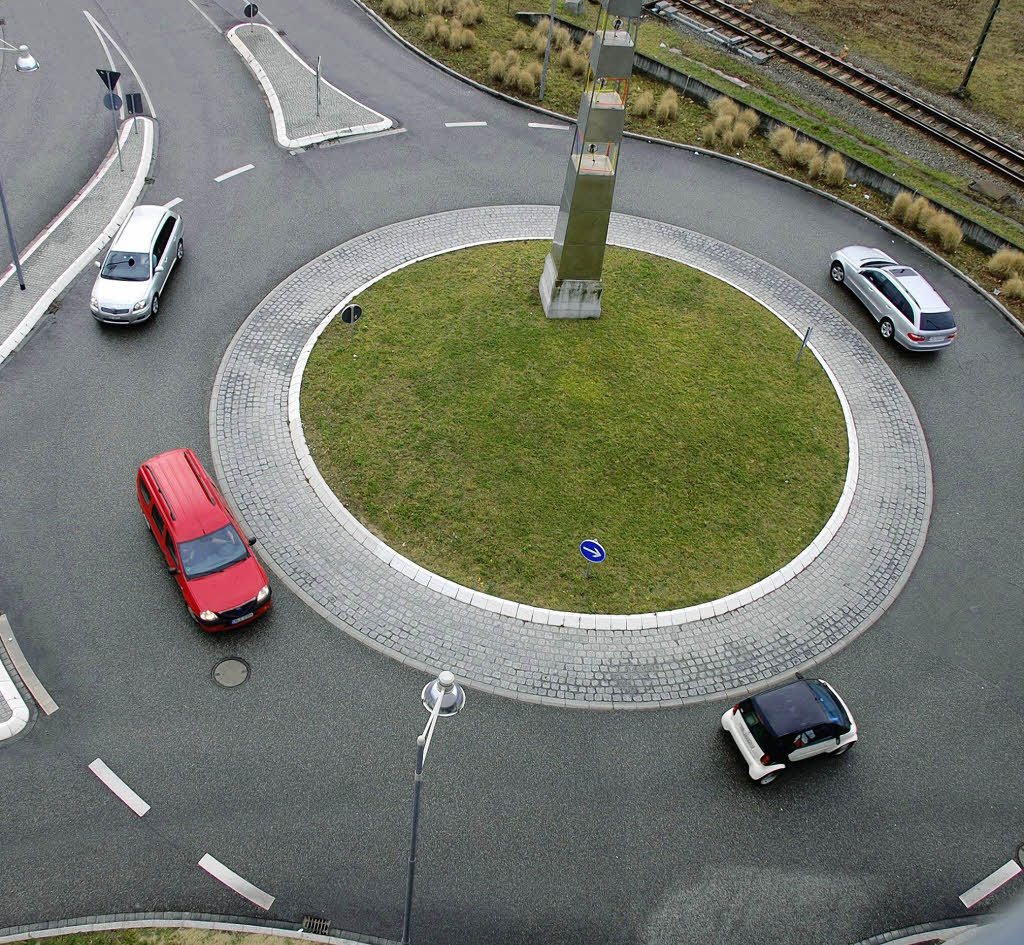
\includegraphics[width=\textwidth,height=0.7\textheight,keepaspectratio]{bilder/54467642.jpg} %http://www.badische-zeitung.de/weil-am-rhein/insel-kreisverkehr-gilt-als-gefaehrlich--54467646.html
\end{center}
\end{frame}

\begin{frame}
	\frametitle{Why Roundabouts}
	\begin{figure}[!ht]
\begin{center}
\caption{Accident Rate in City Limits}
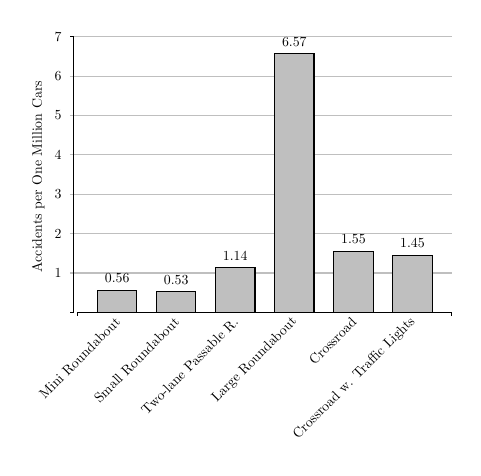
\begin{tikzpicture}[scale=0.5, transform shape]
  \foreach \x in {1,...,7}  %Hilfslinien
    \draw[gray!50, text=black] (-0.2 cm,\x cm) -- (9.5cm,\x cm) 
      node at (-0.5 cm,\x cm) {\x};  %Beschriftung der Hilfslinien
  \draw (0cm,0cm) -- (9.5cm,0cm);  %Abzisse
  \draw (0cm,0cm) -- (0cm,-0.1cm);  %linkes Ende der Abzisse
  \draw (9.5cm,0cm) -- (9.5cm,-0.1cm);  %rechtes Ende der Abzisse
  \draw (-0.1cm,0cm) -- (-0.1cm,7.0cm);  %Ordinate
  \draw (-0.1cm,0cm) -- (-0.2cm,0cm);  %unteres Ende der Ordinate
  \draw (-0.1cm,7.0cm) -- (-0.2cm,7.0cm);  %oberes Ende der Ordinate
  \node[rotate=90, left] at (-1.0cm,6cm) {Accidents per One Million Cars}; %Säulenbeschriftung
  \foreach \x/\y/\country in {0.5/0.56/Mini Roundabout,  %\x ist Anfang der Säulen
                              2/0.53/Small Roundabout,  %\y ist Höhe der Säulen
                              3.5/1.14/Two-lane Passable R.,
                              5/6.57/Large Roundabout,
                              6.5/1.55/Crossroad,
                              8/1.45/Crossroad w. Traffic Lights}
    {
     \draw[fill=gray!50] (\x cm,0cm) rectangle (1.0cm+\x cm,\y cm) %die Säulen
       node at (0.5cm + \x cm,\y cm + 0.3cm) {\y}; %die Prozente über den Säulen
     \node[rotate=45, left] at (0.6 cm +\x cm,-0.1cm) {\country}; %Säulenbeschriftung
    };
\end{tikzpicture}
\label{accident_rate}
\end{center}
\end{figure}

\end{frame}

\begin{frame}
\frametitle{Why Roundabouts}
\begin{figure}[!ht]
\begin{center}
\caption{Accident Charge Rate in City Limits}
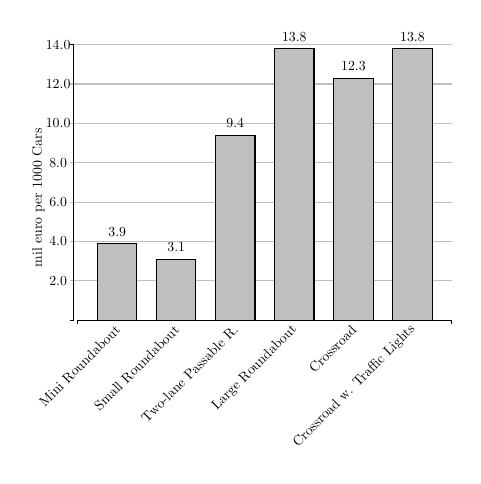
\begin{tikzpicture}[scale=0.5, transform shape]
  \foreach \x in {1,...,7}{  %Hilfslinien
   \pgfmathsetmacro\result{\x *2}
    \draw[gray!50, text=black] (-0.2 cm,\x cm) -- (9.5cm,\x cm) 
      node at (-0.5 cm,\x cm) {\result};  %Beschriftung der Hilfslinien
     }
  \draw (0cm,0cm) -- (9.5cm,0cm);  %Abzisse
  \draw (0cm,0cm) -- (0cm,-0.1cm);  %linkes Ende der Abzisse
  \draw (9.5cm,0cm) -- (9.5cm,-0.1cm);  %rechtes Ende der Abzisse
  \draw (-0.1cm,0cm) -- (-0.1cm,7.0cm);  %Ordinate
  \draw (-0.1cm,0cm) -- (-0.2cm,0cm);  %unteres Ende der Ordinate
  \draw (-0.1cm,7.0cm) -- (-0.2cm,7.0cm);  %oberes Ende der Ordinate
  \node[rotate=90, left] at (-1.0cm,5cm) {mil euro  per 1000 Cars}; %Säulenbeschriftung
  \foreach \x/\y/\value/\country in {0.5/1.95/3.9/Mini Roundabout,  %\x ist Anfang der Säulen
                              2/1.55/3.1/Small Roundabout,  %\y ist Höhe der Säulen
                              3.5/4.7/9.4/Two-lane Passable R.,
                              5/6.9/13.8/Large Roundabout,
                              6.5/6.15/12.3/Crossroad,
                              8/6.9/13.8/Crossroad w. Traffic Lights}
    {
     \draw[fill=gray!50] (\x cm,0cm) rectangle (1.0cm+\x cm,\y cm) %die Säulen
       node at (0.5cm + \x cm,\y cm + 0.3cm) {\value}; %die Prozente über den Säulen
     \node[rotate=45, left] at (0.6 cm +\x cm,-0.1cm) {\country}; %Säulenbeschriftung
    };
\end{tikzpicture}
\label{charge_rate}
\end{center}
\end{figure}
\end{frame}


\begin{frame}
\frametitle{Test Platform}
\begin{figure}[!ht]
%\begin{center}
\caption{Snowfox}
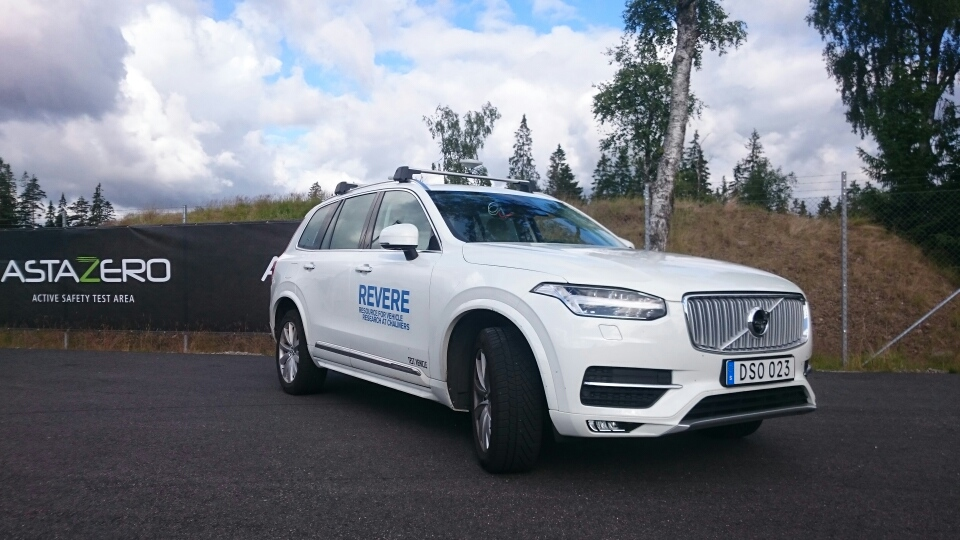
\includegraphics[width=\textwidth,height=0.7\textheight,keepaspectratio]{bilder/snowfox.jpg}
\label{platform}
%\end{center}
\end{figure}
\end{frame}

\begin{frame}
\frametitle{Test Platform}
\begin{figure}[!ht]
%\begin{center}
\caption{Snowfox Sensors}
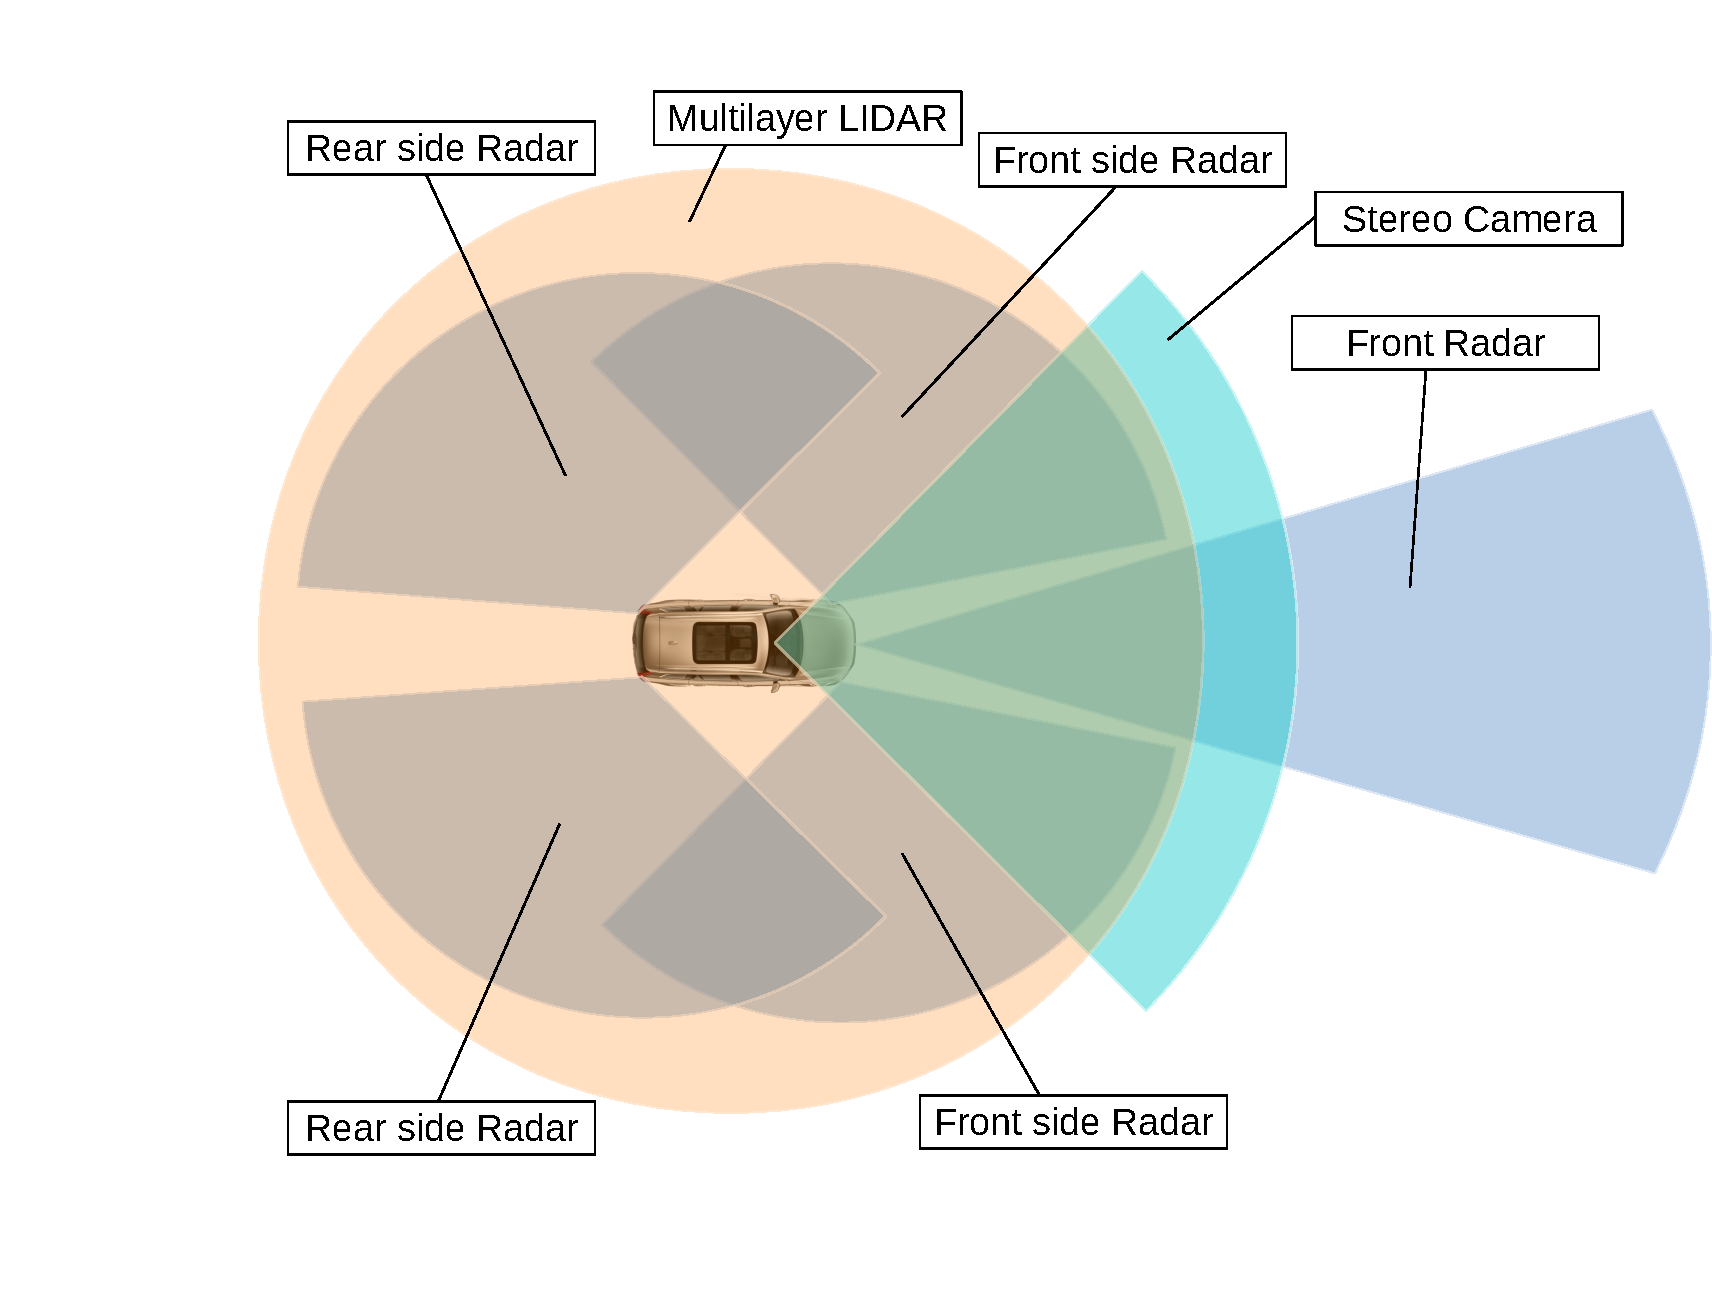
\includegraphics[width=\textwidth,height=0.7\textheight,keepaspectratio]{sensors.pdf}
\label{platform}
%\end{center}
\end{figure}
\end{frame}






\section{Main Problems}
%
\begin{frame}
	\frametitle{Main Problems}
	\begin{itemize}
		\item Object Detection
		\begin{itemize}
			\item Segmentation
			\item Tracking
			\item Classification
		\end{itemize}
		\item Simulation
		\begin{itemize}
			\item Scenario
			\item Logic
		\end{itemize}
		\item Evaluation
		\begin{itemize}
			\item Simulation
			\item Real Measurements
			\item Performance
		\end{itemize}
	\end{itemize}
\end{frame}

\section{Segmentation}

\begin{frame}
\frametitle{Segmentation}
 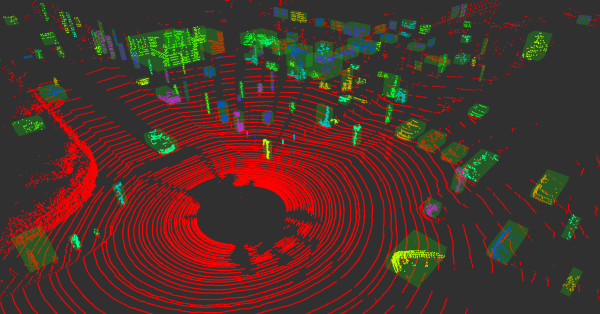
\includegraphics[width=\textwidth,height=0.7\textheight,keepaspectratio]{bilder/segmented_objects.png} 
 %https://www.mrt.kit.edu/mitarbeiter_3401.php
\end{frame}



\begin{frame}
\frametitle{Segmentation - Ground Removal}
\begin{figure}[!ht]
%\begin{center}
\caption{Unsegmented Data}
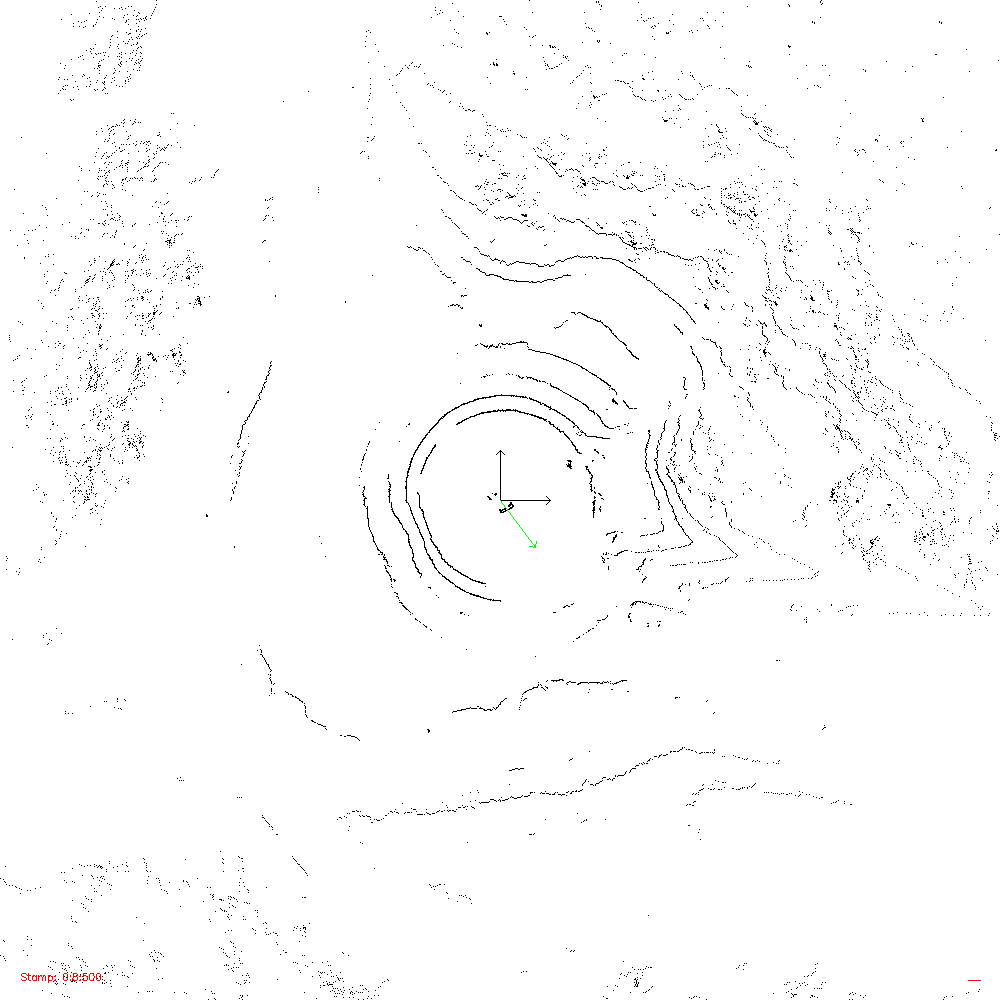
\includegraphics[width=\textwidth,height=0.7\textheight,keepaspectratio]{bilder/before_seg/img100084.png}
\label{segments}
%\end{center}
\end{figure}
\end{frame}

\begin{frame}
\frametitle{Segmentation - Ground Removal}
\begin{figure}[!ht]
%\begin{center}
\caption{Segmented Data}
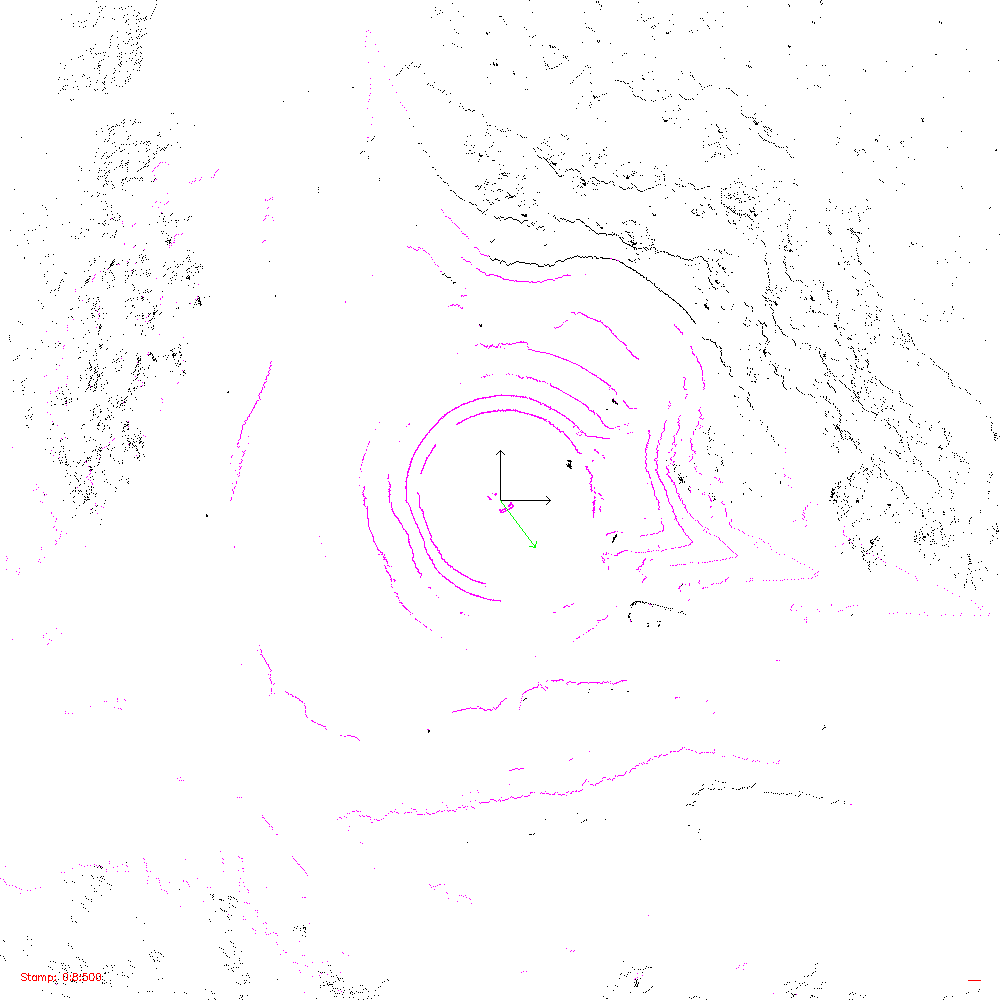
\includegraphics[width=\textwidth,height=0.7\textheight,keepaspectratio]{bilder/Segmentation/img100084.png}
\label{segments}
%\end{center}
\end{figure}
\end{frame}


\begin{frame}
\frametitle{Segmentation - Ground Removal}
\begin{figure}[!ht]
%\begin{center}
\caption{LiDAR Segments}

\includegraphics[width=\textwidth,height=0.7\textheight,keepaspectratio]{bilder/segments.png}
\label{segments}
%\end{center}
\end{figure}
\end{frame}


\begin{frame}
\frametitle{Segmentation - Ground Removal}
\begin{figure}[!ht]
\begin{center}
\caption{RANSAC - Random Sample Consensus}
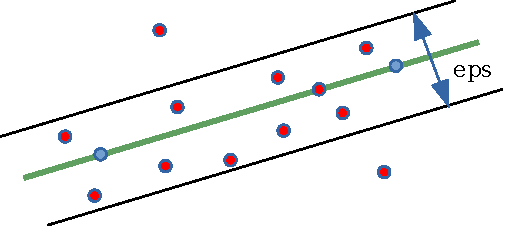
\includegraphics[width=\textwidth,height=0.7\textheight,keepaspectratio]{bilder/ransac.pdf}
\label{ransac}
\end{center}
\end{figure}
\end{frame}

\begin{frame}
\frametitle{Segmentation - Clustering}
\begin{figure}[!ht]
%\begin{center}
\caption{Segmented Data}
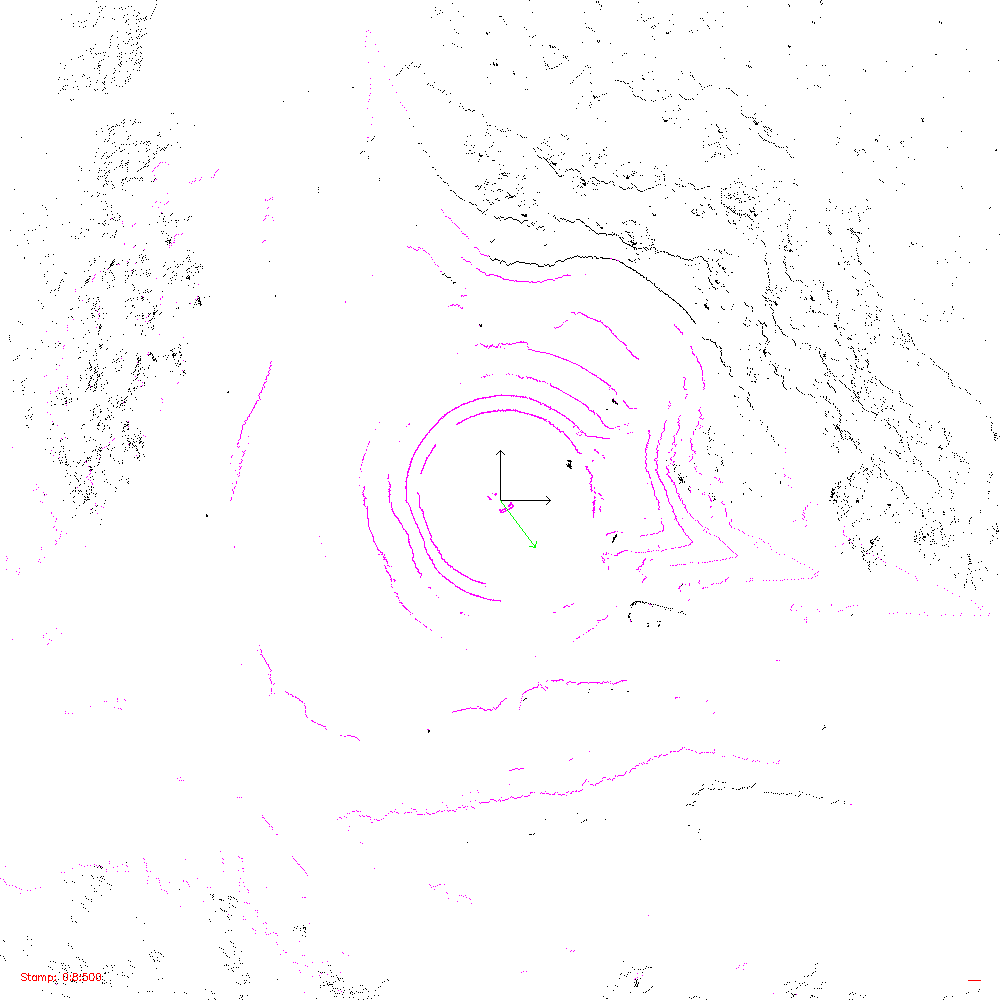
\includegraphics[width=\textwidth,height=0.7\textheight,keepaspectratio]{bilder/Segmentation/img100084.png}
\label{segments}
%\end{center}
\end{figure}
\end{frame}

\begin{frame}
\frametitle{Segmentation - Clustering}
\begin{figure}[!ht]
\begin{center}
\caption{DBSCAN - Density-Based Spatial Clustering with Noise}
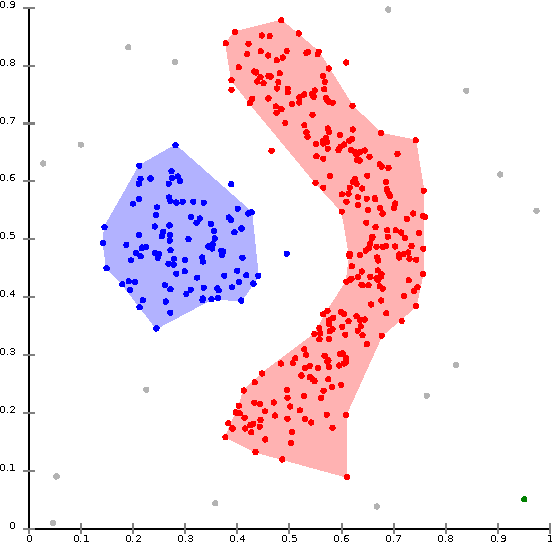
\includegraphics[width=\textwidth,height=0.7\textheight,keepaspectratio]{bilder/DBSCAN-density-data.pdf}%https://en.wikipedia.org/wiki/DBSCAN
\label{dbscan}
\end{center}
\end{figure}
\end{frame}


\section{Tracking}

\begin{frame}
\frametitle{Tracking}
\begin{center}
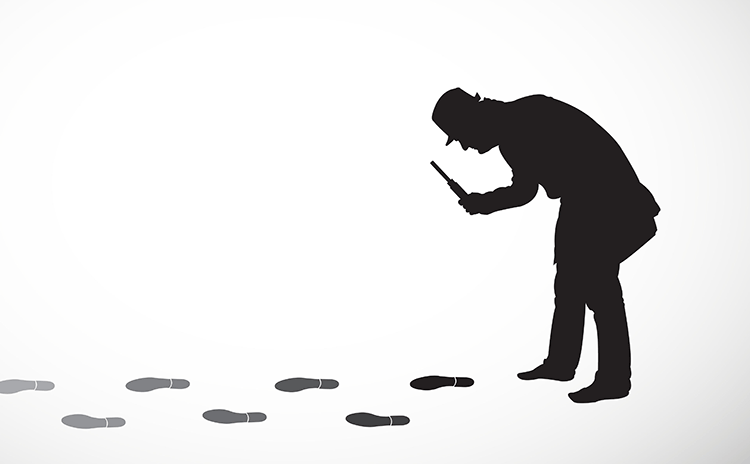
\includegraphics[width=\textwidth,height=0.7\textheight,keepaspectratio]{bilder/detective-tracking.png} %http://www.vehicletrackingexperts.co.uk/is-it-illegal-to-track-your-spouses-or-childs-car/
\end{center}
\end{frame}


\begin{frame}
\frametitle{Tracking}
\begin{figure}[!ht]
%\begin{center}
\caption{Segmented Data}
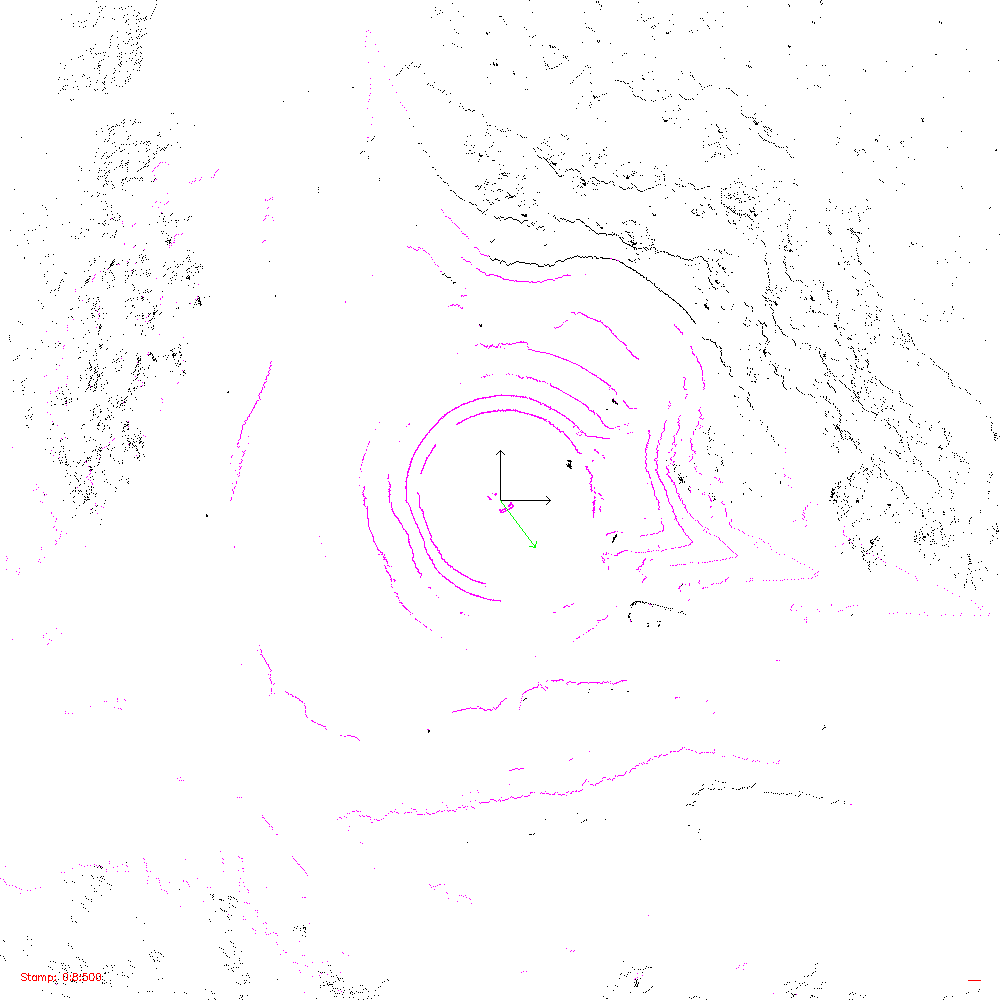
\includegraphics[width=\textwidth,height=0.7\textheight,keepaspectratio]{bilder/Segmentation/img100084.png}
\label{segments}
%\end{center}
\end{figure}
\end{frame}

\begin{frame}
\frametitle{Tracking}
\begin{figure}[!ht]
%\begin{center}
\caption{Segmentation - Segmentation}
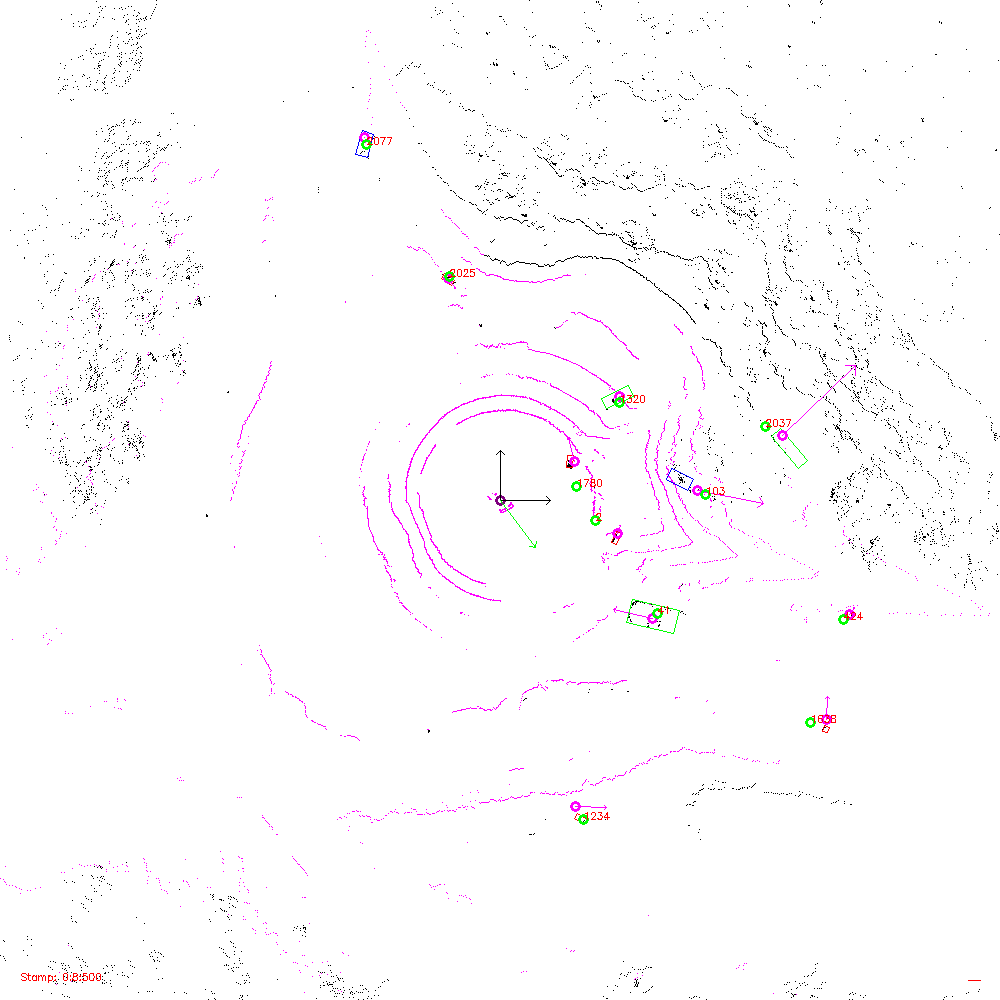
\includegraphics[width=\textwidth,height=0.7\textheight,keepaspectratio]{bilder/clust/img100084.png}
\label{segments}
%\end{center}
\end{figure}
\end{frame}

\begin{frame}
\frametitle{Tracking - Tracking of simplified Clusters}
  \begin{itemize}
    \item clusters are defined through there mean center point
    \item tracking is done through a simple distance criteria    
  \end{itemize}
\end{frame}

\begin{frame}
\frametitle{Tracking - Tracking of simplified Clusters}
  \begin{itemize}
    \item now, we can track the Objects from timestep to timestep
    \item but.. we need more information
    \begin{itemize}
    \item direction and speed of the object movement
    \item prediction of the movement
    \end{itemize}
  \end{itemize}
\end{frame}

\begin{frame}
\frametitle{Tracking - Tracking of simplified Clusters}
\begin{itemize}
    \item calculation oth the movement through:
  \end{itemize}
  \begin{align*}
    \Delta x &= P_x(t) - P_x(t_{-2m}) + \Delta C_x\\
    \Delta y &= P_y(t) - P_y(t_{-2m}) + \Delta C_y\\
    \theta &= \atantwo(\Delta y,\Delta x)
  \end{align*}
\end{frame}



\begin{frame}
\frametitle{Tracking - Tracking of simplified Clusters}
\begin{figure}[!ht]
%\begin{center}
\caption{Direction of movement}
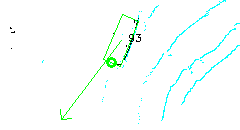
\includegraphics[width=\textwidth,height=0.7\textheight,keepaspectratio]{bilder/obst_rot.png}
\label{segments}
%\end{center}
\end{figure}
\end{frame}


\begin{frame}
\frametitle{Tracking - How to Calculate Bounding Boxes}
\begin{figure}[!ht]
%\begin{center}
\caption{Minimum Bounding Box}
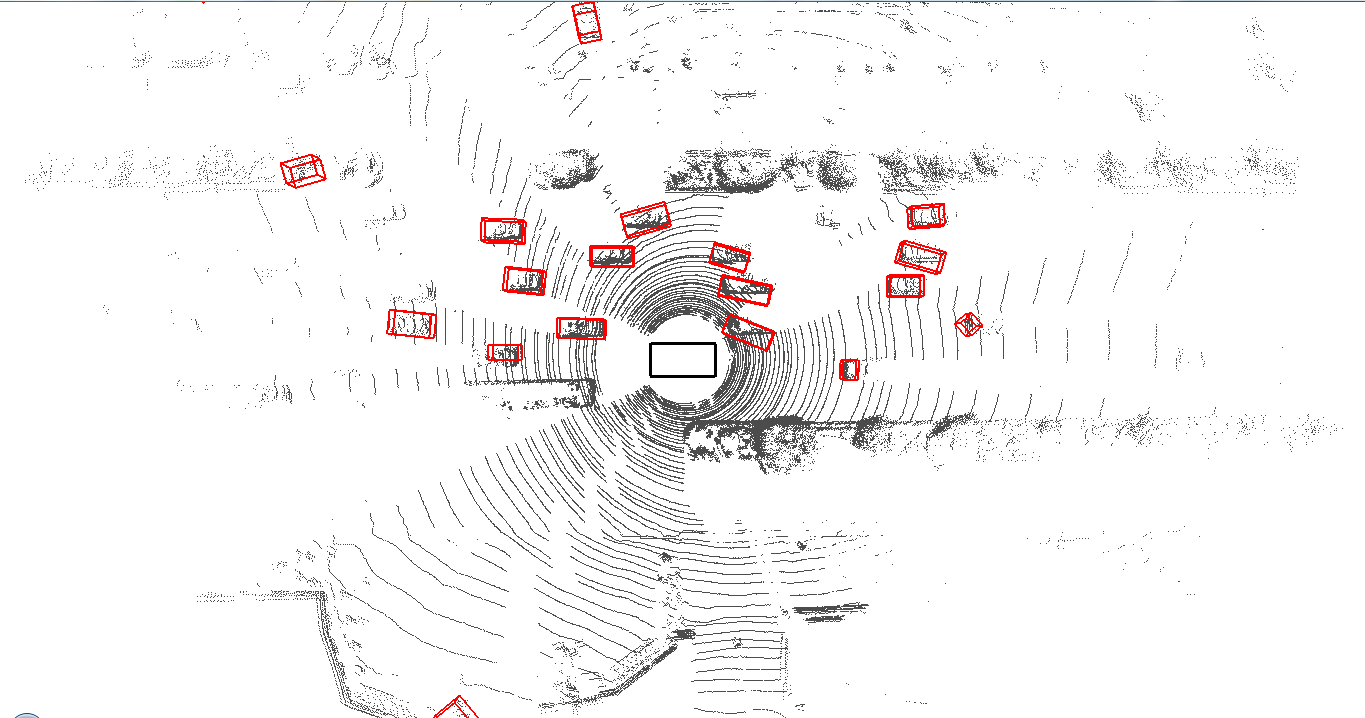
\includegraphics[width=\textwidth,height=0.7\textheight,keepaspectratio]{bilder/min_bound_wrong.png}
\label{segments}
%\end{center}
\end{figure}
\end{frame}


\begin{frame}
\frametitle{Tracking - How to Calculate Bounding Boxes}
\begin{figure}[!ht]
%\begin{center}
\caption{Object Rotation and Division}
\begin{tabular}{ l r }
 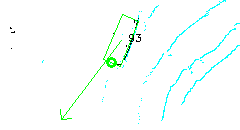
\includegraphics[width=0.45\textwidth,height=0.7\textheight,keepaspectratio]{bilder/obst_rot.png} &
 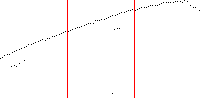
\includegraphics[width=0.45\textwidth,height=0.7\textheight,keepaspectratio]{bilder/obst_devide.png}
\end{tabular}
\label{segments}
%\end{center}
\end{figure}
\end{frame}



\begin{frame}
\frametitle{Tracking - How to Calculate Bounding Boxes}
\begin{figure}[!ht]
%\begin{center}
\caption{Maximize Y-Values}
\begin{tabular}{ l r }
 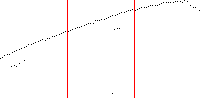
\includegraphics[width=0.45\textwidth,height=0.7\textheight,keepaspectratio]{bilder/obst_devide.png} &
 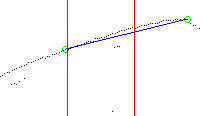
\includegraphics[width=0.45\textwidth,height=0.7\textheight,keepaspectratio]{bilder/obst_devide_angle.png}
\end{tabular}
\label{segments}
%\end{center}
\end{figure}
\end{frame}

\begin{frame}
\frametitle{Tracking - How to Calculate Bounding Boxes}
\begin{figure}[!ht]
%\begin{center}
\caption{Calculating Correction}
\begin{tabular}{ l r }
 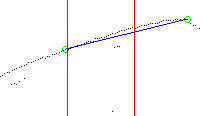
\includegraphics[width=0.45\textwidth,height=0.7\textheight,keepaspectratio]{bilder/obst_devide_angle.png} &
 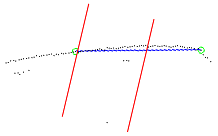
\includegraphics[width=0.45\textwidth,height=0.7\textheight,keepaspectratio]{bilder/obst_devide_angle_rot.png}
\end{tabular}
\begin{align*}
\Delta x &= R_x - L_x\\
\Delta y &= R_y - L_y\\
\theta_{correction} &= \atantwo(\Delta y,\Delta x)
\end{align*}
\label{segments}
%\end{center}
\end{figure}
\end{frame}


\begin{frame}
\frametitle{Tracking - Size calculation}
\begin{figure}[!ht]
%\begin{center}
\caption{Size Calculation}
\begin{tabular}{ l r }
 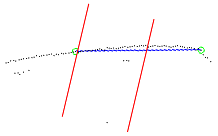
\includegraphics[width=0.45\textwidth,height=0.7\textheight,keepaspectratio]{bilder/obst_devide_angle_rot.png} &
 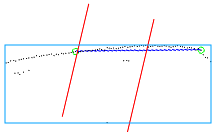
\includegraphics[width=0.45\textwidth,height=0.7\textheight,keepaspectratio]{bilder/obst_devide_angle_size.png}
\end{tabular}
\label{segments}
%\end{center}
\end{figure}
\end{frame}

\begin{frame}
\frametitle{Tracking - Size calculation}
\begin{figure}[!ht]
\begin{center}
\caption{Bounding Box Calculation Cases}
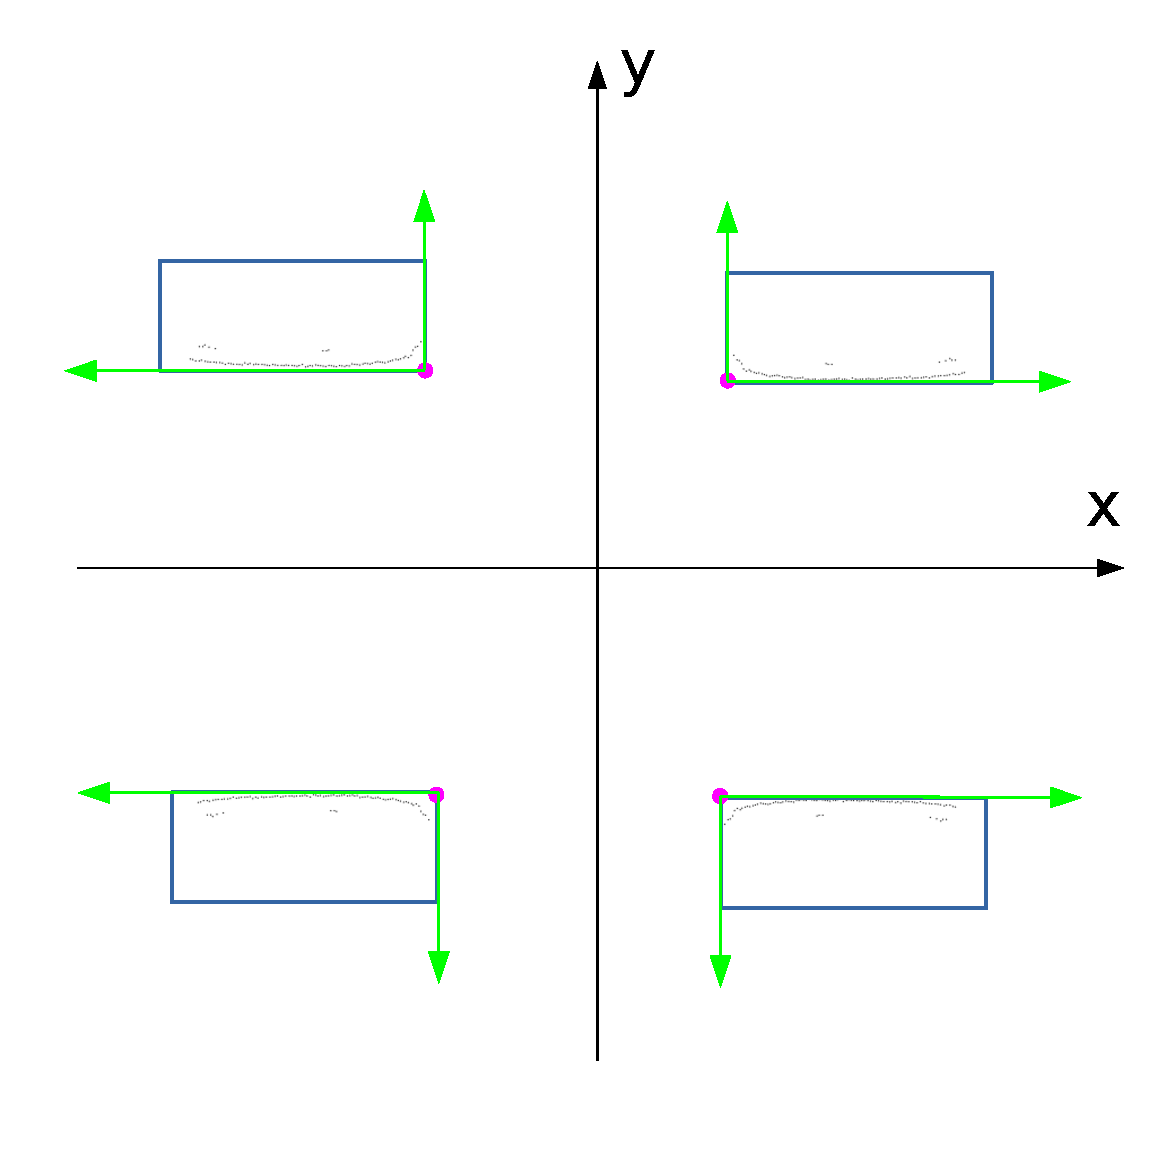
\includegraphics[width=\textwidth,height=0.7\textheight,keepaspectratio]{bilder/cases.pdf}
\label{obst_cases}
\end{center}
\end{figure}
\end{frame}



\begin{frame}
\frametitle{Tracking - Size calculation}

\begin{figure}[!ht]
\begin{center}
\caption{Object Size Histogram}
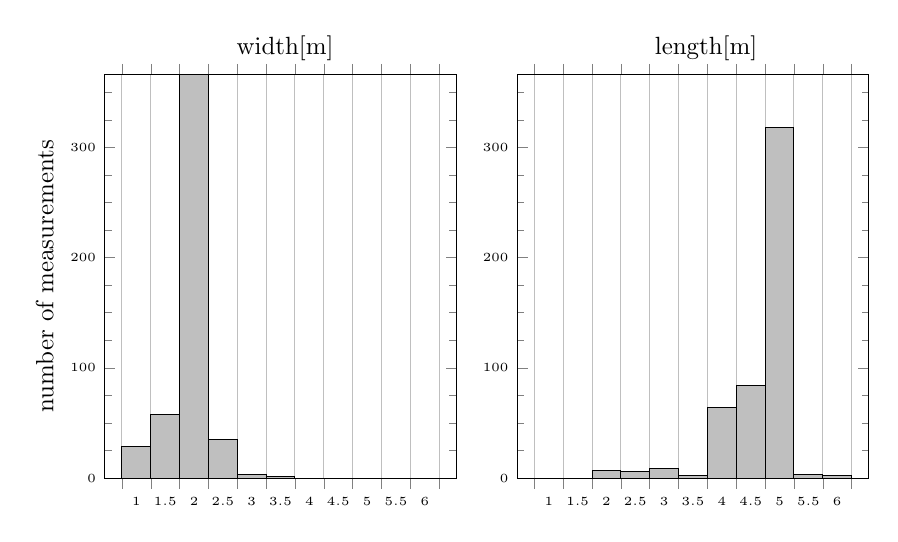
\begin{tikzpicture}[scale=0.9, transform shape]
\begin{axis}[ylabel={number of measurements},ybar interval, ymax=366,ymin=0,xmin=0.7,xmax=6.8, minor y tick num = 3, width=0.54\textwidth, height=0.6\textwidth, ticklabel style = {font=\tiny}]
\addplot[fill=gray!50] coordinates { (1.0, 29) (1.5, 58) (2.0, 366) (2.5, 35) (3.0, 3) (3.5, 1) (4.0, 0) (4.5, 0) (5.0, 0) (5.5, 0) (6.0, 0) (6.5, 0) };
\end{axis}
\begin{axis}[ybar interval, ymax=366,ymin=0,xmin=0.7,xmax=6.8, minor y tick num = 3, width=0.54\textwidth, height=0.6\textwidth, at={(0.48\textwidth,0)}, ticklabel style = {font=\tiny}]
\addplot[fill=gray!50] coordinates { (1.0, 0) (1.5, 0) (2.0, 7) (2.5, 6) (3.0, 9) (3.5, 2) (4.0, 64) (4.5, 84) (5.0, 318) (5.5, 3) (6.0, 2) (6.5, 2) };
\end{axis}
\node at (0.21\textwidth,0.5\textwidth) {width[m]};
\node at (0.7\textwidth,0.5\textwidth) {length[m]};
\end{tikzpicture}
\label{obst_hist}
\end{center}
\end{figure}

\end{frame}


\begin{frame}
\frametitle{Tracking - Confidence}
Increase confidence value by one, if the object could be tracked and

\begin{itemize}
\item The width of the object is less than the length of the obstacle plus 1.5m
\item The length of the obstacle is less than 10m
\item The width of the obstacle less less than 4m
\end{itemize}

and halved if not

\end{frame}


\section{Classification}

\begin{frame}
\frametitle{Classification}
Using simple size based approach

\begin{description}
\item[pedestrian:] length < 1.5 m and width < 1.5 m
\item[cyclist:] length < 2 m and width < 1.5 m
\item[car:] length < 10 m and width < 4 m
\item[undefined:] length >= 10 m and width >= 4 m
\end{description}

\end{frame}


\section{State Estimation}	


\begin{frame}
\frametitle{State Estimation}
using constant turn rate and velocity model and extendet Kalman filter

\begin{align*}
\vec{x}(t) &=
\begin{bmatrix}
x & y & \theta & v & \omega
\end{bmatrix}^T\\
x &\text{ - x-Axis}\\
y &\text{ - y-Axis}\\
\theta &\text{ - Object Yaw Angle}\\
v &\text{ - Object Velocity}\\
\omega &\text{ - Yaw Rate}
\end{align*}

\end{frame}


\begin{frame}
\frametitle{State Estimation - Extendet Kalman Filter}
\begin{align*}
f = \vec{x}(t + \Delta t)=
\begin{bmatrix}
\frac{v}{\omega} (-\sin(\theta) + \sin(\Delta t \omega + \theta)) + x(t) \\
\frac{v}{\omega} (\cos(\theta) - cos(\Delta t \omega + \theta)) + y(t) \\
\omega \Delta t + \theta\\
v\\
\omega
\end{bmatrix} 
\end{align*}
\begin{itemize}
\item a lot more equations..
\item hacks for numerical stability (yawrate near zero)
\item singularity in rotation (because $[- 180^{\circ} \le \theta \le 180^{\circ}] $)
\end{itemize}

\end{frame}


\begin{frame}
\frametitle{State Estimation - Extendet Kalman Filter}

\begin{itemize}
\item filtering the data
\item prediction of the future position if an object could not be detected in a timestep
\item reassigning in case of redetection, using the predicted position
\end{itemize}


\end{frame}

\section{Simulation}

\begin{frame}
\frametitle{Simulation}
\begin{figure}[!ht]
\begin{center}
\caption{Simulation - Scenario}
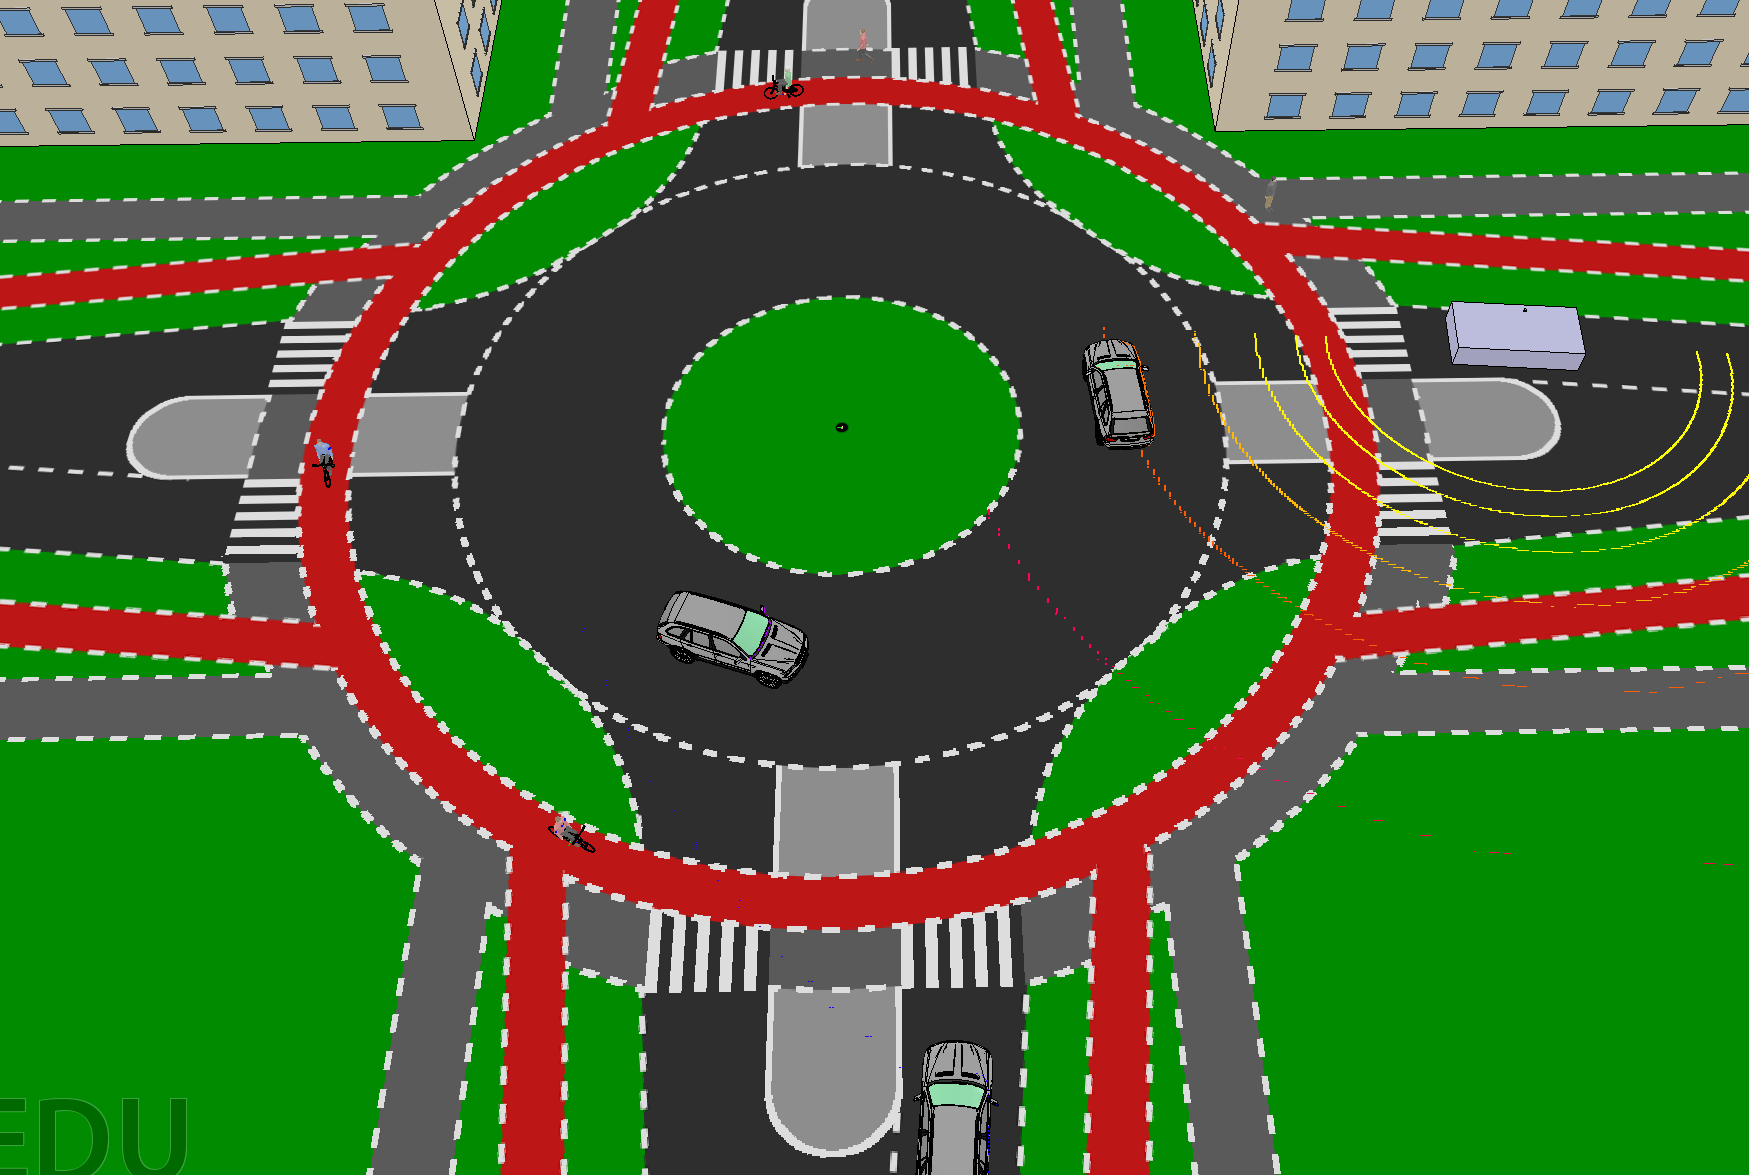
\includegraphics[width=\textwidth,height=0.7\textheight,keepaspectratio]{bilder/scenario.png}
\label{obst_cases}
\end{center}
\end{figure}
\end{frame}


\begin{frame}
\frametitle{Mapping}
\begin{figure}[!ht]
\begin{center}
 \begin{tikzpicture}[scale=0.9, transform shape]
  \umlclass{ROAD}{
  roadid : int \\
  roadname : string \\
  lanes : lane[]}{}
  \umlclass[x=6,y=0]{LANE}{
  laneid : int \\
  width : float \\
  type : string \\
  leftlanemarking : string\\
  rightlanemarking : string\\
  lanemodel : pointmodel\\
  connections : tuple[]
  }{}
  \umlclass[x=6,y=-4]{POINTMODEL}{
  points : VERTEX2[]
  }{}
  \umlclass[x=0,y=-4]{VERTEX2}{
  points : float[2]
  }{}
  \umlunicompo[mult=1..*]{ROAD}{LANE}
  \umlunicompo{LANE}{POINTMODEL}
  \umlunicompo[mult=2..*]{POINTMODEL}{VERTEX2}
  \end{tikzpicture}
\end{center}
\end{figure}
\end{frame}

\begin{frame}
\frametitle{Mapping}
\begin{figure}[!ht]
\begin{center}
 \begin{tikzpicture}[scale=0.9, transform shape]
  \umlclass{ROUNDABOUT}{
  roundaboutid : int \\
  lanes : lane[]\\
  junctions : tuple[]\\
  inner\_lane\_radius : float[]\\
  outer\_lane\_radius : float[]\\
  center :  VERTEX2
  }{}
  \end{tikzpicture}
\end{center}
\end{figure}
\end{frame}

\begin{frame}
\frametitle{Mapping}
\begin{figure}[!ht]
\begin{center}
\caption{Mapping - Lanesegment}
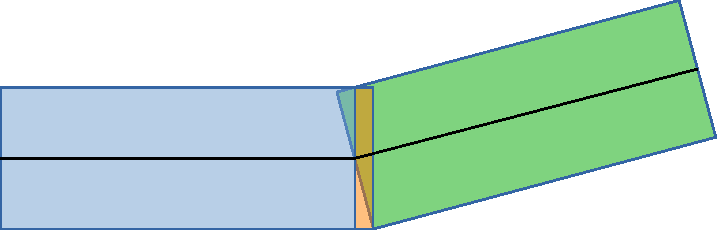
\includegraphics[width=0.9\textwidth,height=0.7\textheight,keepaspectratio]{bilder/mapping.pdf}
\end{center}
\end{figure}
\end{frame}


\begin{frame}
\frametitle{State Machine}
\begin{figure}[!ht]
\begin{center}
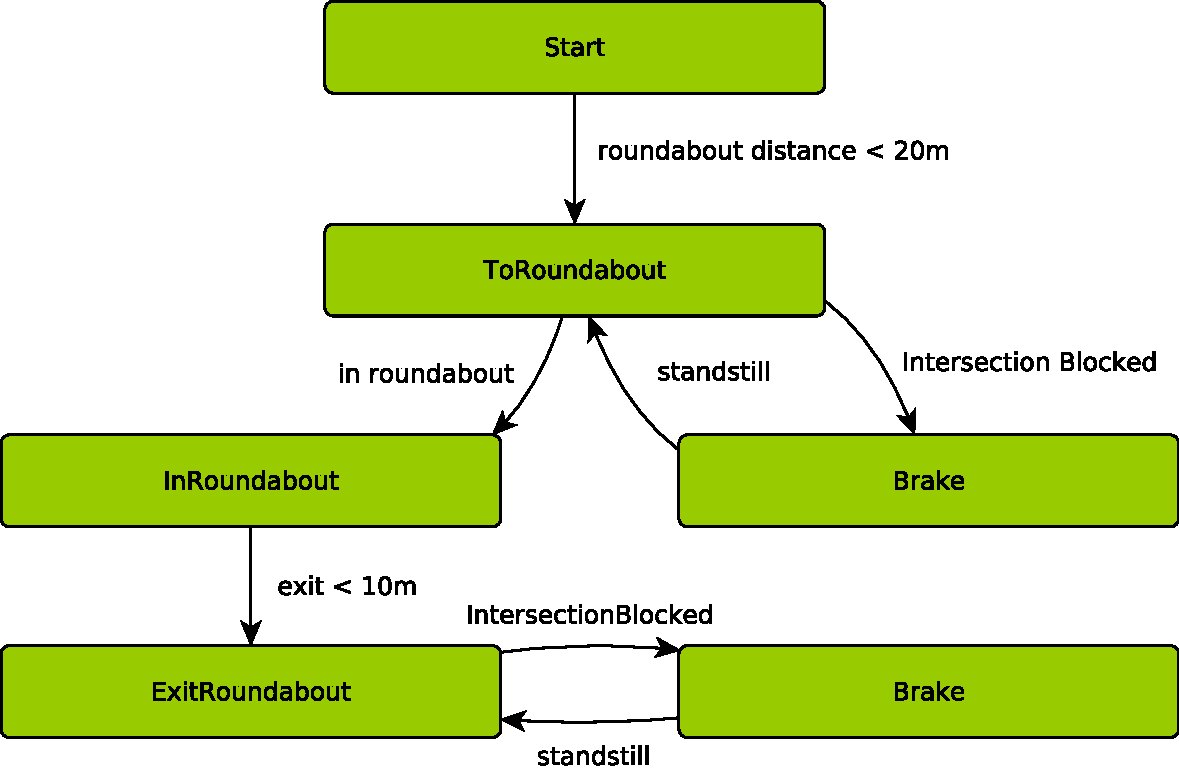
\includegraphics[width=\textwidth,height=0.7\textheight,keepaspectratio]{bilder/stateMachine.pdf}
\end{center}
\end{figure}
\end{frame}

\begin{frame}
\frametitle{Simulation}
\begin{figure}[!ht]
\begin{center}
\caption{Simulation - Intersection Position}
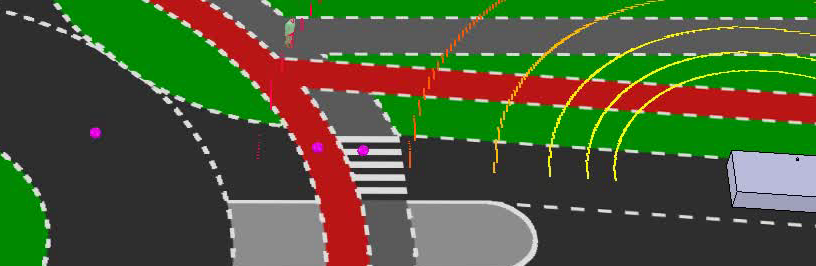
\includegraphics[width=\textwidth,height=0.7\textheight,keepaspectratio]{bilder/intersection_pos.png}
\label{obst_cases}
\end{center}
\end{figure}
\end{frame}


\section{Evaluation}

\begin{frame}
\frametitle{Evaluation}
\begin{figure}[!ht]
\begin{center}
  \caption{Detection Distance Performance} 
    \centering
    \begin{minipage}[t]{0.49\textwidth}
        \centering
        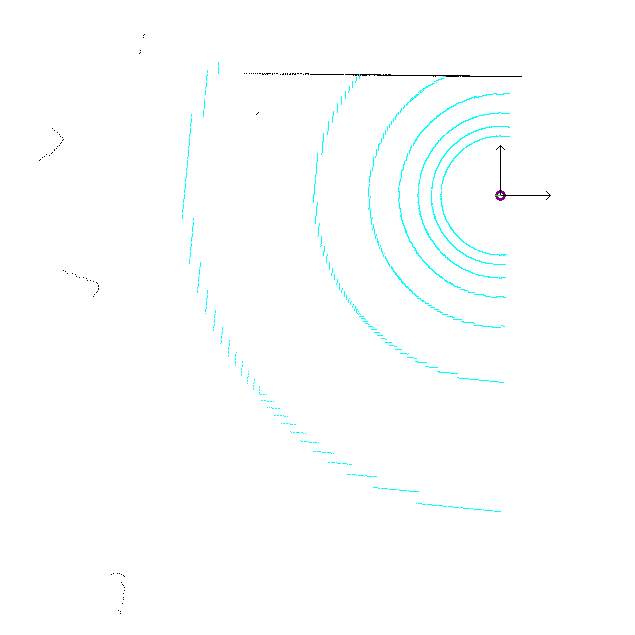
\includegraphics[width=\textwidth]{bilder/alg/img100001_s.png}\\
        Timestep 1
    \end{minipage}% <- sonst wird hier ein Leerzeichen eingefügt
    \hfill
    \begin{minipage}[t]{0.49\textwidth}
        \centering
	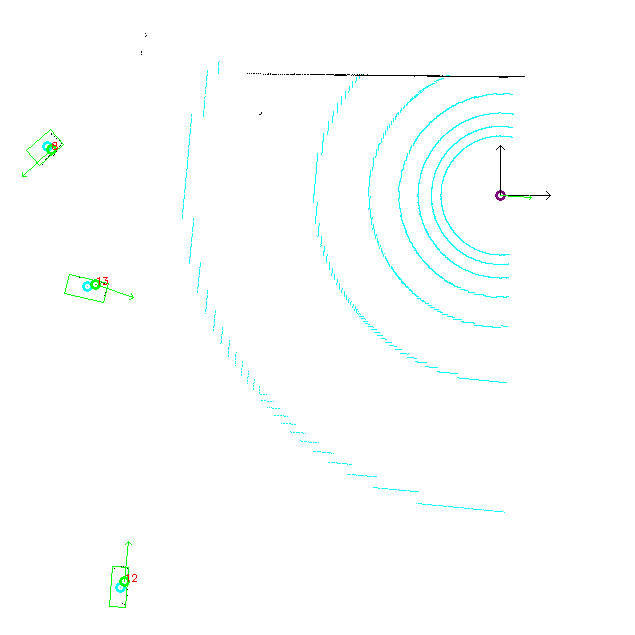
\includegraphics[width=\textwidth]{bilder/alg/img100002_s.png}\\
        Timestep 2
    \end{minipage}
    \label{detection_performance}
\label{obst_cases}
\end{center}
\end{figure}
\end{frame}


\begin{frame}
\frametitle{Evaluation}
\begin{figure}[!ht]
\begin{center}
\caption{Detection Distance Performance Pedestrians/Cyclists}
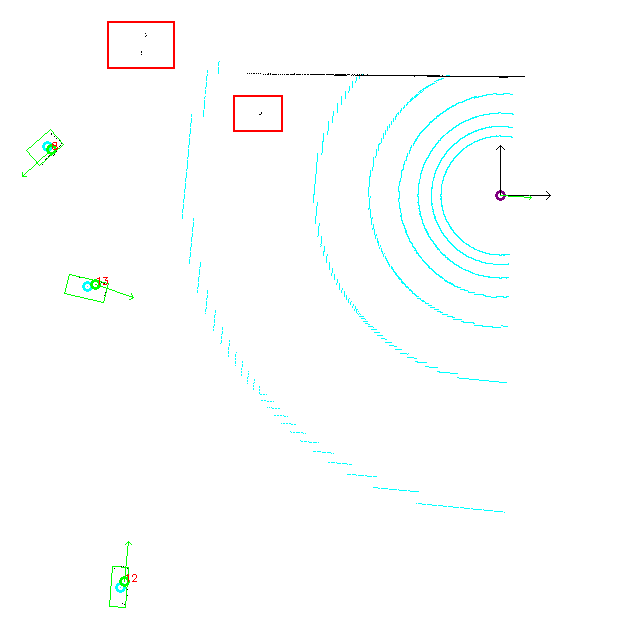
\includegraphics[width=\textwidth,height=0.7\textheight,keepaspectratio]{bilder/alg/img100002_m_s.png}
\label{obst_cases}
\end{center}
\end{figure}
\end{frame}

\begin{frame}
\frametitle{Evaluation}
\begin{figure}[!ht]
\begin{center}
\caption{Car Position Error}
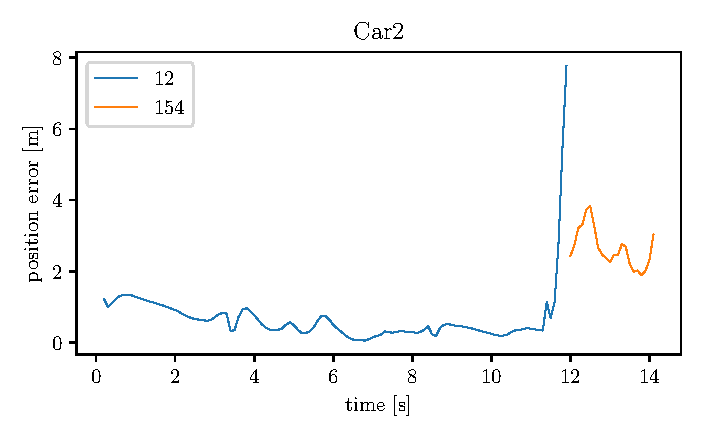
\includegraphics[width=\textwidth,height=0.7\textheight,keepaspectratio]{bilder/Car2_pos_err.pdf}
\label{obst_cases}
\end{center}
\end{figure}
\end{frame}

\begin{frame}
\frametitle{Evaluation}
\begin{figure}[!ht]
\begin{center}
\caption{Tracking Error}

    \begin{minipage}[t]{0.49\textwidth}
        \centering
        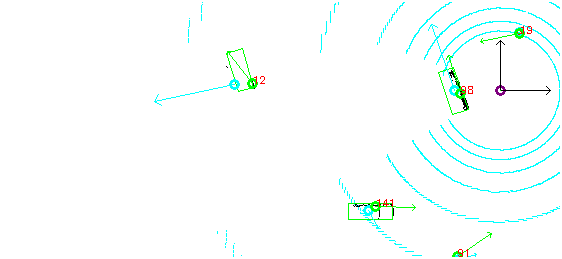
\includegraphics[width=\textwidth]{bilder/alg/lost_wob.png}
    \end{minipage}% <- sonst wird hier ein Leerzeichen eingefügt
    \hfill
    \begin{minipage}[t]{0.49\textwidth}
        \centering
	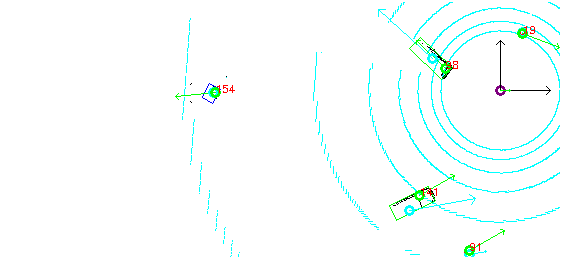
\includegraphics[width=\textwidth]{bilder/alg/redetect_wob.png}
    \end{minipage}
\label{obst_cases}
\end{center}
\end{figure}
\end{frame}

\begin{frame}
\frametitle{Evaluation}
\begin{figure}[!ht]
\begin{center}
\caption{Car Position Error / Distance}
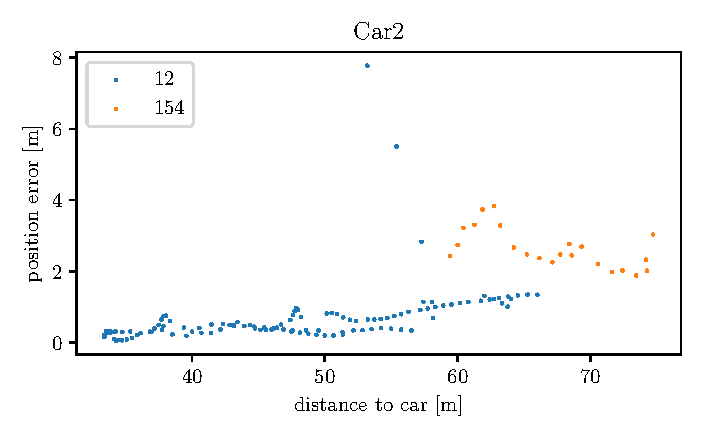
\includegraphics[width=\textwidth,height=0.7\textheight,keepaspectratio]{bilder/Car2_pos_err_dist.pdf}
\label{obst_cases}
\end{center}
\end{figure}
\end{frame}


\begin{frame}
\frametitle{Evaluation}
\begin{figure}[!ht]
\begin{center}
\caption{Simulation Sensor Resolution}
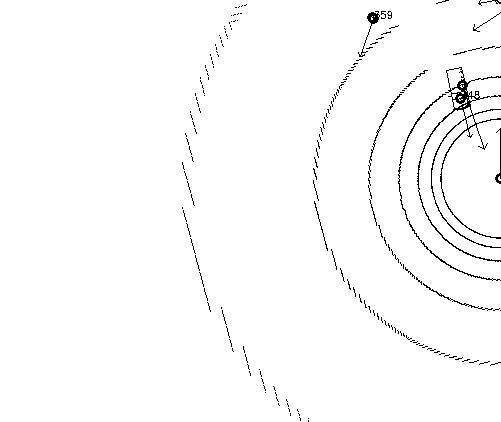
\includegraphics[width=\textwidth,height=0.7\textheight,keepaspectratio]{bilder/sen_err.png}
\label{obst_cases}
\end{center}
\end{figure}
\end{frame}

\begin{frame}
\frametitle{Evaluation}
\begin{figure}[!ht]
\begin{center}
\caption{Speed}
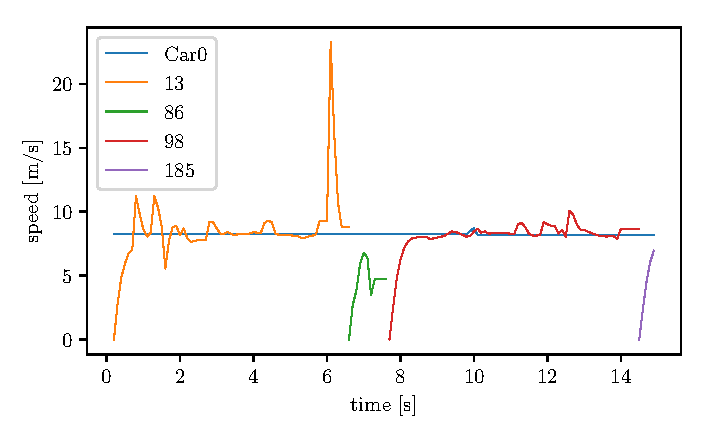
\includegraphics[width=\textwidth,height=0.7\textheight,keepaspectratio]{bilder/Car0_speed.pdf}
\label{obst_cases}
\end{center}
\end{figure}
\end{frame}

\begin{frame}
\frametitle{Evaluation}
\begin{figure}[!htb]
  \caption{Classification} 
  \centering
  \begin{tabularx}{\textwidth}{X|r|r|r|r}
  \hline \textbf{Name} & \textbf{Car [\%]} & \textbf{Bike [\%]} & \textbf{Pedestrian [\%]} & \textbf{UnCl [\%]} \\\hline
    Pedestrian & 0 & 0 & 100 & 0 \\\hline
    Car0 & 100 & 0 & 0 & 0 \\\hline
    Car1 & 100 & 0 & 0 & 0 \\\hline
    Car2 & 98.2 & 0.73 & 0.98 & 0 \\\hline
    Bike0 & 0 & 0.5 & 99.5 & 0 \\\hline
    Bike1 & 0 & 0 & 100 & 0 \\\hline
    Bike2 & 1.9 & 1.2 & 96.9 & 0 \\
  \end{tabularx}
 \label{classification}
\end{figure}
\end{frame}


\begin{frame}
\frametitle{Evaluation}
\begin{figure}[htb]
  \caption{Confidence Filtering} 
    \centering
    \begin{minipage}[t]{0.49\textwidth}
        \centering
          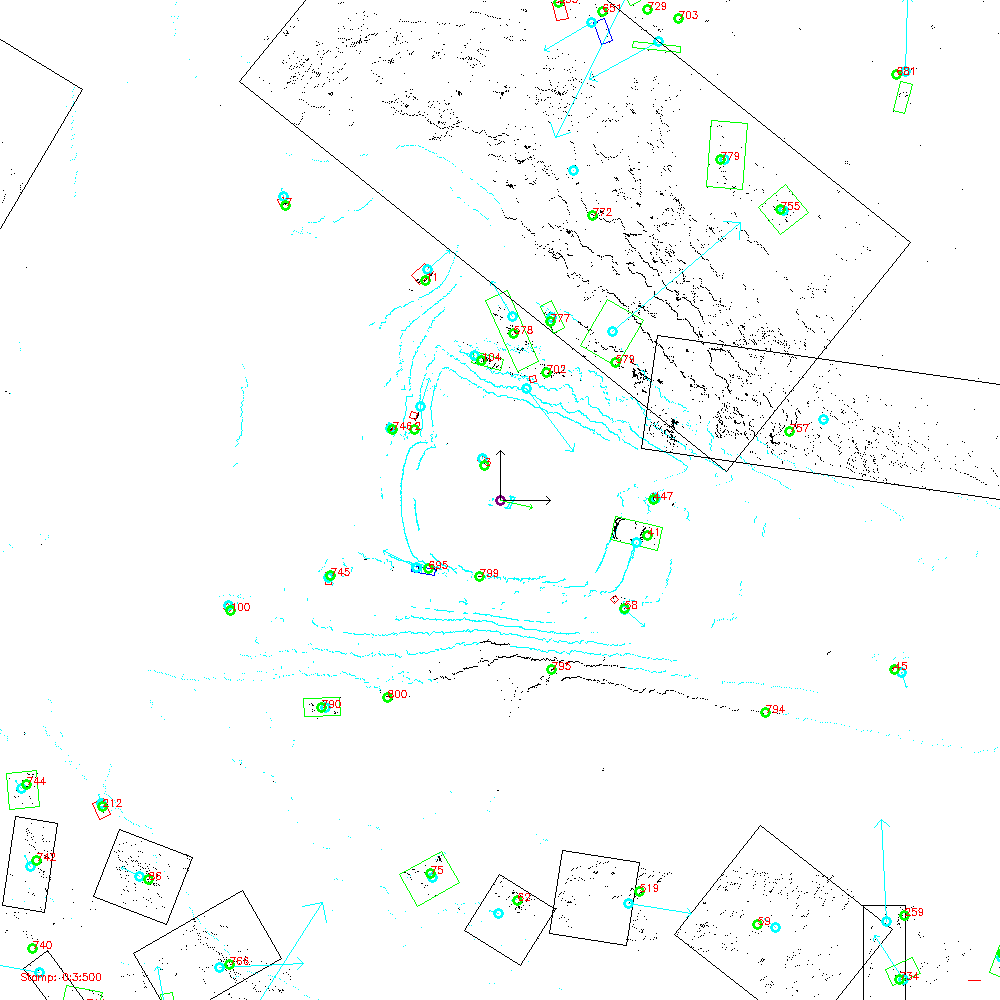
\includegraphics[width=\textwidth]{bilder/filter_off.png}\\
          without filtering
    \end{minipage}% <- sonst wird hier ein Leerzeichen eingefügt
    \hfill
    \begin{minipage}[t]{0.49\textwidth}
        \centering
	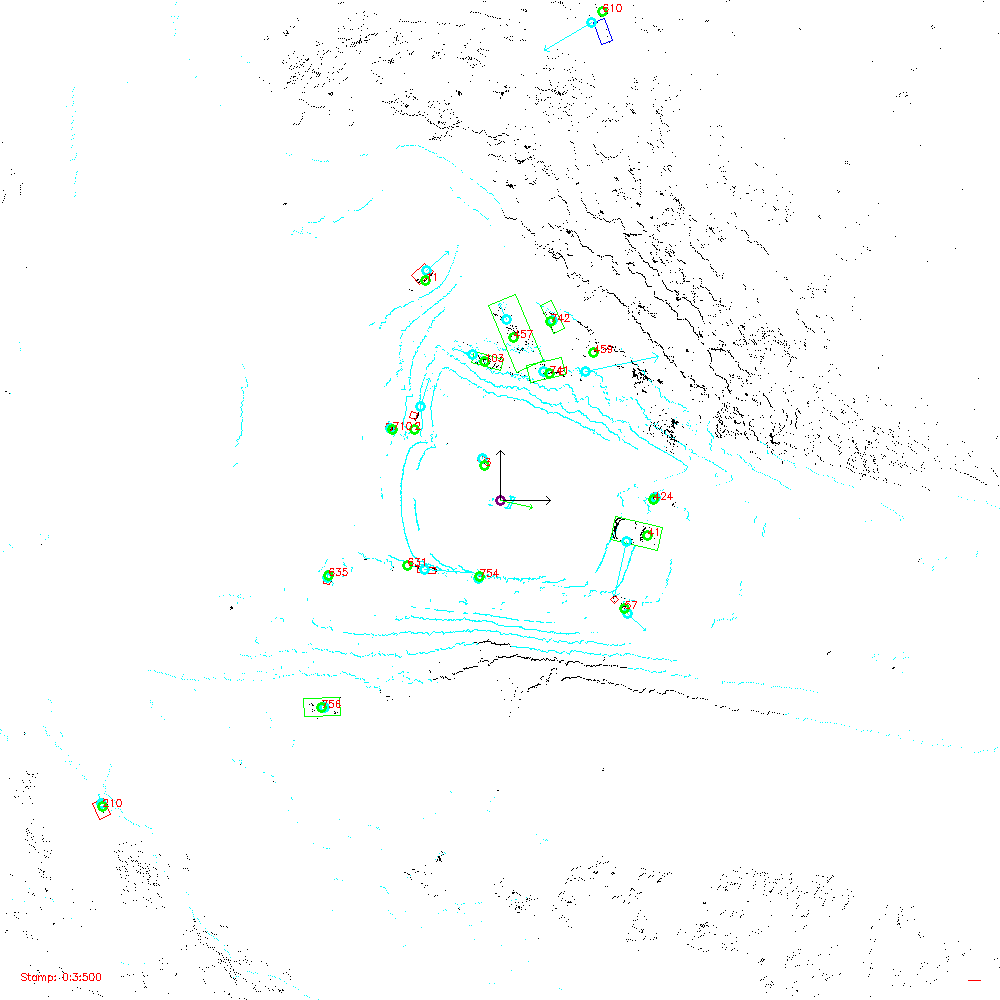
\includegraphics[width=\textwidth]{bilder/filter_on.png}\\
	with filtering
    \end{minipage}
    \label{conf_filter}
\end{figure}
\end{frame}




\begin{frame}
\frametitle{Evaluation}
\begin{figure}[!ht]
\begin{center}
\caption{Reflector Posts }
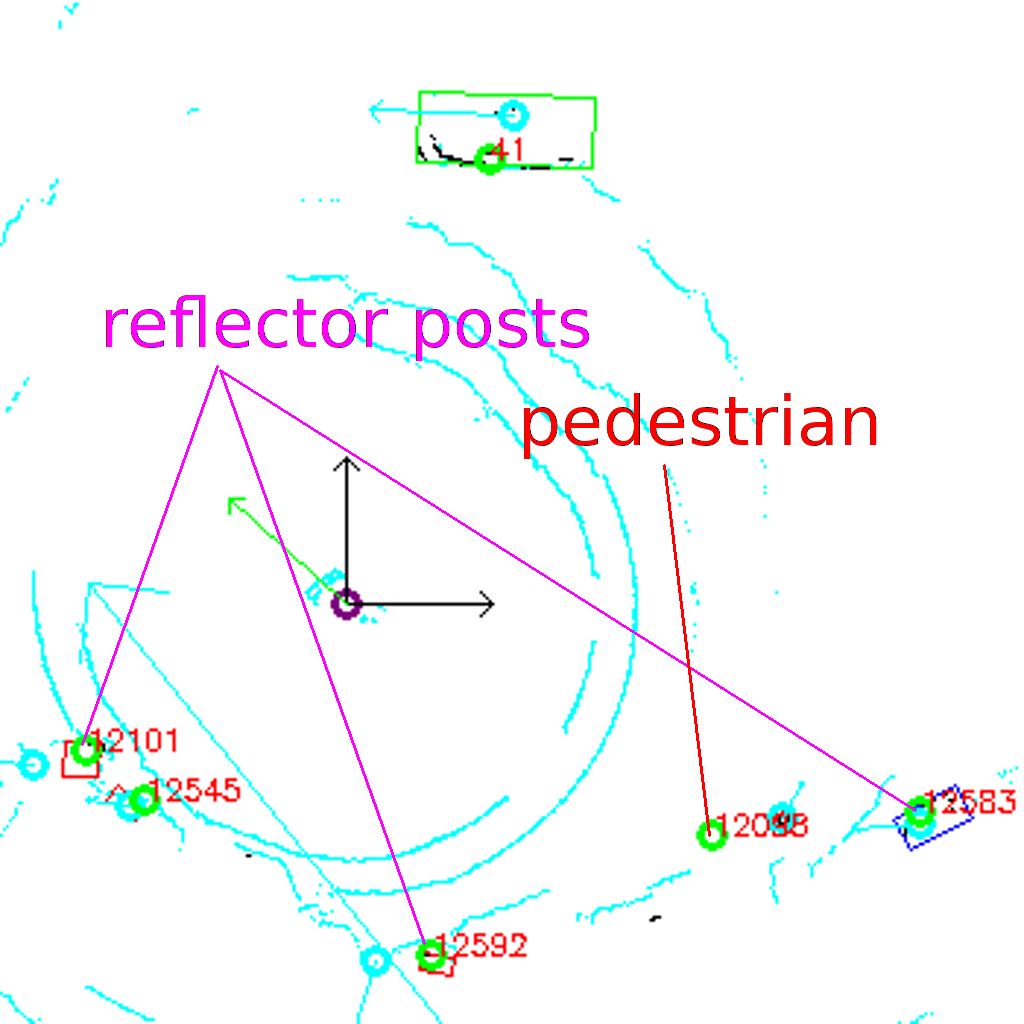
\includegraphics[width=\textwidth,height=0.7\textheight,keepaspectratio]{bilder/reflector_posts.png}
\label{obst_cases}
\end{center}
\end{figure}
\end{frame}


\begin{frame}
\frametitle{Evaluation}
\begin{figure}[!ht]
\begin{center}
\caption{Performance}
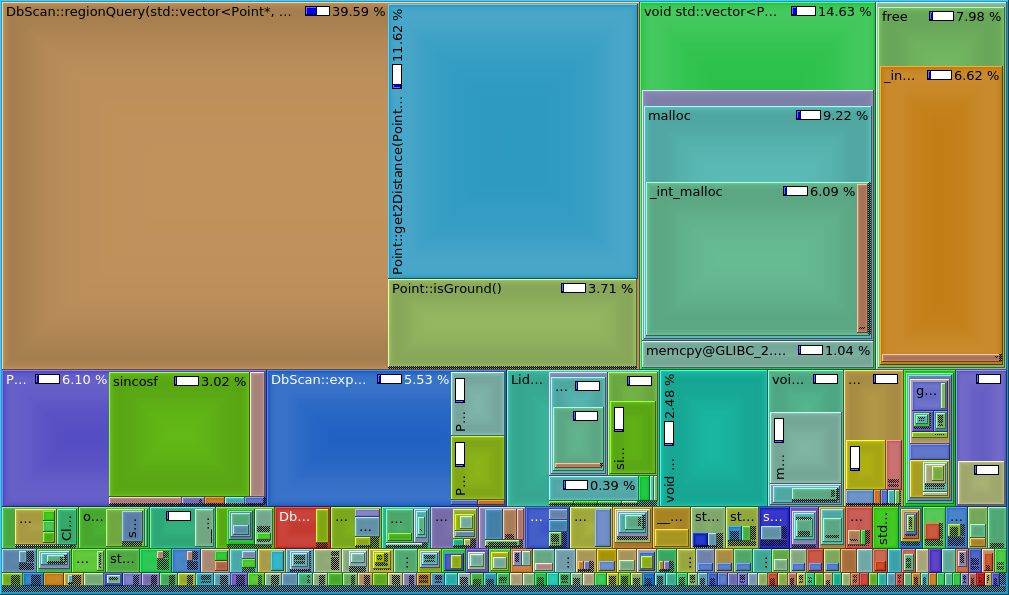
\includegraphics[width=\textwidth,height=0.7\textheight,keepaspectratio]{bilder/call.png}
\label{obst_cases}
\end{center}
\end{figure}
\end{frame}




\addtocounter{framenumber}{-1}
\begin{frame}[plain]
	
	\titlepage
\end{frame}
%
\end{document}
